% Slide 5
\begin{frame}[fragile]
\frametitle{Core Operation}

\begin{figure}
\caption{\texttt{afl} Input Queue}
\begin{center}
{\scalefont{0.9}
\scalebox{0.65}{% Graphic for TeX using PGF
% Title: /home/nskinkel/queue.dia
% Creator: Dia v0.97.3
% CreationDate: Mon Apr 18 17:12:26 2016
% For: nskinkel
% \usepackage{tikz}
% The following commands are not supported in PSTricks at present
% We define them conditionally, so when they are implemented,
% this pgf file will use them.
\ifx\du\undefined
  \newlength{\du}
\fi
\setlength{\du}{15\unitlength}
\begin{tikzpicture}
\pgftransformxscale{1.000000}
\pgftransformyscale{-1.000000}
\definecolor{dialinecolor}{rgb}{0.000000, 0.000000, 0.000000}
\pgfsetstrokecolor{dialinecolor}
\definecolor{dialinecolor}{rgb}{1.000000, 1.000000, 1.000000}
\pgfsetfillcolor{dialinecolor}
\pgfsetlinewidth{0.100000\du}
\pgfsetdash{}{0pt}
\pgfsetdash{}{0pt}
\pgfsetmiterjoin
\definecolor{dialinecolor}{rgb}{1.000000, 1.000000, 1.000000}
\pgfsetfillcolor{dialinecolor}
\fill (5.000000\du,5.000000\du)--(5.000000\du,7.000000\du)--(7.000000\du,7.000000\du)--(7.000000\du,5.000000\du)--cycle;
\definecolor{dialinecolor}{rgb}{0.882353, 0.000000, 0.000000}
\pgfsetstrokecolor{dialinecolor}
\draw (5.000000\du,5.000000\du)--(5.000000\du,7.000000\du)--(7.000000\du,7.000000\du)--(7.000000\du,5.000000\du)--cycle;
\pgfsetlinewidth{0.100000\du}
\pgfsetdash{}{0pt}
\pgfsetdash{}{0pt}
\pgfsetmiterjoin
\definecolor{dialinecolor}{rgb}{1.000000, 1.000000, 1.000000}
\pgfsetfillcolor{dialinecolor}
\fill (7.000000\du,5.000000\du)--(7.000000\du,7.000000\du)--(9.000000\du,7.000000\du)--(9.000000\du,5.000000\du)--cycle;
\definecolor{dialinecolor}{rgb}{0.882353, 0.000000, 0.000000}
\pgfsetstrokecolor{dialinecolor}
\draw (7.000000\du,5.000000\du)--(7.000000\du,7.000000\du)--(9.000000\du,7.000000\du)--(9.000000\du,5.000000\du)--cycle;
\pgfsetlinewidth{0.100000\du}
\pgfsetdash{}{0pt}
\pgfsetdash{}{0pt}
\pgfsetmiterjoin
\definecolor{dialinecolor}{rgb}{1.000000, 1.000000, 1.000000}
\pgfsetfillcolor{dialinecolor}
\fill (9.000000\du,5.000000\du)--(9.000000\du,7.000000\du)--(11.000000\du,7.000000\du)--(11.000000\du,5.000000\du)--cycle;
\definecolor{dialinecolor}{rgb}{0.882353, 0.000000, 0.000000}
\pgfsetstrokecolor{dialinecolor}
\draw (9.000000\du,5.000000\du)--(9.000000\du,7.000000\du)--(11.000000\du,7.000000\du)--(11.000000\du,5.000000\du)--cycle;
\pgfsetlinewidth{0.100000\du}
\pgfsetdash{}{0pt}
\pgfsetdash{}{0pt}
\pgfsetmiterjoin
\definecolor{dialinecolor}{rgb}{1.000000, 1.000000, 1.000000}
\pgfsetfillcolor{dialinecolor}
\fill (11.000000\du,5.000000\du)--(11.000000\du,7.000000\du)--(13.000000\du,7.000000\du)--(13.000000\du,5.000000\du)--cycle;
\definecolor{dialinecolor}{rgb}{0.882353, 0.000000, 0.000000}
\pgfsetstrokecolor{dialinecolor}
\draw (11.000000\du,5.000000\du)--(11.000000\du,7.000000\du)--(13.000000\du,7.000000\du)--(13.000000\du,5.000000\du)--cycle;
% setfont left to latex
\definecolor{dialinecolor}{rgb}{0.000000, 0.000000, 0.000000}
\pgfsetstrokecolor{dialinecolor}
\node[anchor=west] at (5.300000\du,6.000000\du){$T_1$};
\pgfsetlinewidth{0.100000\du}
\pgfsetdash{}{0pt}
\pgfsetdash{}{0pt}
\pgfsetbuttcap
\pgfsetmiterjoin
\pgfsetlinewidth{0.100000\du}
\pgfsetbuttcap
\pgfsetmiterjoin
\pgfsetdash{}{0pt}
\definecolor{dialinecolor}{rgb}{0.403922, 0.580392, 0.972549}
\pgfsetfillcolor{dialinecolor}
\pgfpathmoveto{\pgfpoint{14.360799\du}{9.154056\du}}
\pgfpathcurveto{\pgfpoint{14.050939\du}{9.141219\du}}{\pgfpoint{13.450000\du}{9.410813\du}}{\pgfpoint{13.534507\du}{9.988517\du}}
\pgfpathcurveto{\pgfpoint{13.619014\du}{10.566220\du}}{\pgfpoint{14.022770\du}{10.694593\du}}{\pgfpoint{14.191785\du}{10.527706\du}}
\pgfpathcurveto{\pgfpoint{14.360799\du}{10.360814\du}}{\pgfpoint{13.928873\du}{11.336486\du}}{\pgfpoint{14.755166\du}{11.593243\du}}
\pgfpathcurveto{\pgfpoint{15.581451\du}{11.850000\du}}{\pgfpoint{16.003988\du}{11.439189\du}}{\pgfpoint{15.881922\du}{11.143918\du}}
\pgfpathcurveto{\pgfpoint{15.759856\du}{10.848648\du}}{\pgfpoint{16.604928\du}{11.837162\du}}{\pgfpoint{16.999295\du}{11.272297\du}}
\pgfpathcurveto{\pgfpoint{17.393662\du}{10.707431\du}}{\pgfpoint{16.595538\du}{10.168247\du}}{\pgfpoint{16.764553\du}{10.245274\du}}
\pgfpathcurveto{\pgfpoint{16.933567\du}{10.322301\du}}{\pgfpoint{17.450000\du}{10.219598\du}}{\pgfpoint{17.280986\du}{9.256759\du}}
\pgfpathcurveto{\pgfpoint{17.111971\du}{8.293920\du}}{\pgfpoint{15.590841\du}{9.038516\du}}{\pgfpoint{15.759856\du}{8.897299\du}}
\pgfpathcurveto{\pgfpoint{15.928870\du}{8.756083\du}}{\pgfpoint{15.506334\du}{8.050000\du}}{\pgfpoint{14.980519\du}{8.191216\du}}
\pgfpathcurveto{\pgfpoint{14.454696\du}{8.332434\du}}{\pgfpoint{14.417400\du}{8.588690\du}}{\pgfpoint{14.361062\du}{9.153556\du}}
\pgfpathlineto{\pgfpoint{14.360799\du}{9.154056\du}}
\pgfusepath{fill}
\definecolor{dialinecolor}{rgb}{0.000000, 0.000000, 0.000000}
\pgfsetstrokecolor{dialinecolor}
\pgfpathmoveto{\pgfpoint{14.360799\du}{9.154056\du}}
\pgfpathcurveto{\pgfpoint{14.050939\du}{9.141219\du}}{\pgfpoint{13.450000\du}{9.410813\du}}{\pgfpoint{13.534507\du}{9.988517\du}}
\pgfpathcurveto{\pgfpoint{13.619014\du}{10.566220\du}}{\pgfpoint{14.022770\du}{10.694593\du}}{\pgfpoint{14.191785\du}{10.527706\du}}
\pgfpathcurveto{\pgfpoint{14.360799\du}{10.360814\du}}{\pgfpoint{13.928873\du}{11.336486\du}}{\pgfpoint{14.755166\du}{11.593243\du}}
\pgfpathcurveto{\pgfpoint{15.581451\du}{11.850000\du}}{\pgfpoint{16.003988\du}{11.439189\du}}{\pgfpoint{15.881922\du}{11.143918\du}}
\pgfpathcurveto{\pgfpoint{15.759856\du}{10.848648\du}}{\pgfpoint{16.604928\du}{11.837162\du}}{\pgfpoint{16.999295\du}{11.272297\du}}
\pgfpathcurveto{\pgfpoint{17.393662\du}{10.707431\du}}{\pgfpoint{16.595538\du}{10.168247\du}}{\pgfpoint{16.764553\du}{10.245274\du}}
\pgfpathcurveto{\pgfpoint{16.933567\du}{10.322301\du}}{\pgfpoint{17.450000\du}{10.219598\du}}{\pgfpoint{17.280986\du}{9.256759\du}}
\pgfpathcurveto{\pgfpoint{17.111971\du}{8.293920\du}}{\pgfpoint{15.590841\du}{9.038516\du}}{\pgfpoint{15.759856\du}{8.897299\du}}
\pgfpathcurveto{\pgfpoint{15.928870\du}{8.756083\du}}{\pgfpoint{15.506334\du}{8.050000\du}}{\pgfpoint{14.980519\du}{8.191216\du}}
\pgfpathcurveto{\pgfpoint{14.454696\du}{8.332434\du}}{\pgfpoint{14.417400\du}{8.588690\du}}{\pgfpoint{14.361062\du}{9.153556\du}}
\pgfpathlineto{\pgfpoint{14.360799\du}{9.154056\du}}
\pgfusepath{stroke}
% setfont left to latex
\definecolor{dialinecolor}{rgb}{1.000000, 1.000000, 1.000000}
\pgfsetstrokecolor{dialinecolor}
\node at (15.557226\du,10.216986\du){fuzz};
\pgfsetlinewidth{0.100000\du}
\pgfsetdash{}{0pt}
\pgfsetdash{}{0pt}
\pgfsetbuttcap
{
\definecolor{dialinecolor}{rgb}{0.000000, 0.000000, 0.000000}
\pgfsetfillcolor{dialinecolor}
% was here!!!
\pgfsetarrowsstart{latex}
\definecolor{dialinecolor}{rgb}{0.000000, 0.000000, 0.000000}
\pgfsetstrokecolor{dialinecolor}
\pgfpathmoveto{\pgfpoint{15.958211\du}{8.810151\du}}
\pgfpatharc{10}{-102}{2.458001\du and 2.458001\du}
\pgfusepath{stroke}
}
\pgfsetlinewidth{0.100000\du}
\pgfsetdash{{\pgflinewidth}{0.200000\du}}{0cm}
\pgfsetdash{{\pgflinewidth}{0.200000\du}}{0cm}
\pgfsetbuttcap
{
\definecolor{dialinecolor}{rgb}{0.000000, 0.000000, 0.000000}
\pgfsetfillcolor{dialinecolor}
% was here!!!
\pgfsetarrowsstart{latex}
\definecolor{dialinecolor}{rgb}{0.000000, 0.000000, 0.000000}
\pgfsetstrokecolor{dialinecolor}
\pgfpathmoveto{\pgfpoint{6.446191\du}{7.048492\du}}
\pgfpatharc{153}{79}{6.766308\du and 6.766308\du}
\pgfusepath{stroke}
}
\pgfsetlinewidth{0.100000\du}
\pgfsetdash{{\pgflinewidth}{0.200000\du}}{0cm}
\pgfsetdash{{\pgflinewidth}{0.200000\du}}{0cm}
\pgfsetbuttcap
{
\definecolor{dialinecolor}{rgb}{0.000000, 0.000000, 0.000000}
\pgfsetfillcolor{dialinecolor}
% was here!!!
\pgfsetarrowsend{latex}
\definecolor{dialinecolor}{rgb}{0.000000, 0.000000, 0.000000}
\pgfsetstrokecolor{dialinecolor}
\draw (17.313391\du,9.924906\du)--(21.450000\du,9.900000\du);
}
% setfont left to latex
\definecolor{dialinecolor}{rgb}{0.000000, 0.000000, 0.000000}
\pgfsetstrokecolor{dialinecolor}
\node[anchor=west] at (11.200000\du,5.950000\du){$T_n$};
% setfont left to latex
\definecolor{dialinecolor}{rgb}{0.000000, 0.000000, 0.000000}
\pgfsetstrokecolor{dialinecolor}
\node[anchor=west] at (7.450000\du,6.100000\du){...};
% setfont left to latex
\definecolor{dialinecolor}{rgb}{0.000000, 0.000000, 0.000000}
\pgfsetstrokecolor{dialinecolor}
\node[anchor=west] at (9.525000\du,6.175000\du){...};
% setfont left to latex
\definecolor{dialinecolor}{rgb}{0.000000, 0.000000, 0.000000}
\pgfsetstrokecolor{dialinecolor}
\node[anchor=west] at (17.900000\du,9.400000\du){Discard};
% setfont left to latex
\definecolor{dialinecolor}{rgb}{0.000000, 0.000000, 0.000000}
\pgfsetstrokecolor{dialinecolor}
\node[anchor=west] at (6.700000\du,10.750000\du){Input};
% setfont left to latex
\definecolor{dialinecolor}{rgb}{0.000000, 0.000000, 0.000000}
\pgfsetstrokecolor{dialinecolor}
\node[anchor=west] at (15.600000\du,6.650000\du){Test Case};
\end{tikzpicture}
}
}
\end{center}
\end{figure}

\begin{columns}[c]

\column{0.5\textwidth}

\begin{itemize}
    \item Pruned test case input queue
    \item Spawn new cow processes
    \item Save unique crashes and hangs
\end{itemize}

\column{0.5\textwidth}

\begin{figure}
\caption{\texttt{cow} Process Clones}
\begin{center}
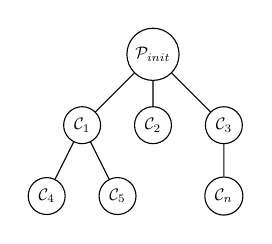
\begin{tikzpicture}[scale=0.6, every node/.style={scale=0.6}]
\node[circle,draw](z){$\mathcal{P}_{init}$}
	child{ node[circle,draw]{$\mathcal{C}_1$} child{node[circle,draw]{$\mathcal{C}_4$}} child{node[circle,draw]{$\mathcal{C}_5$}}}
	child{ node[circle,draw]{$\mathcal{C}_2$} }
	child{ node[circle,draw]{$\mathcal{C}_3$} child{node[circle,draw]{$\mathcal{C}_n$}}};
\end{tikzpicture}
\end{center}
\end{figure}

\end{columns}
\end{frame}
